\begin{quote}
L'intero progetto è stato sviluppato cercando di seguire
il pattern architetturale \emph{modello-vista-controllo} (i.e. \emph{model-view-contoller o MVC}), e cercando di rispettare i principi SOLID.
\end{quote}
\begin{figure}
\centering{
\begin{forest}
	my label/.style={
		label={[font=\sffamily]right:{#1}},
	},
	for tree={
		folder,
		font=\sffamily,
		text=black,
		minimum height=0.45cm,
		text width=40mm,
		rounded corners=4pt,
		grow'=0,
		edge={black,rounded corners,line width=0.5pt},
		fit=band,
	},
	[it.uniud.ducktypesystem, color=SkyBlue
		[\textbf{controller}, color={violet}
			[logger
			]
		]
		[\textbf{distributed}, color={red}
			[data
			]
			[errors
			]
			[impl
			]
			[messages
			]
		]
		[\textbf{view}, color={blue}
		]
		[DucktypeSystem {\color{OliveGreen}$\triangleright$ (Main)}
		]
	]
\end{forest}
\caption{Descrizione del pattern architetturale utilizzato. La cartella \emph{distributed} rappresenta il modulo \emph{model} nel pattern MVC. }
}
\end{figure}

\subsection{Implementazione del sistema distribuito}
\label{sec:akka}
L'ambiente di sviluppo è stato scelto in modo da poter
evidenziare solamente le caratteristiche più rilevanti del problema.
Il sistema è stato implementato in \emph{Akka}, un toolkit costituito da un 
insieme di librerie \emph{open source} per la progettazione e creazione
di sistemi distribuiti e concorrenti, con supporto alla scalabilità e alla
\emph{fault tollerance}, eseguibile su una JVM.
Il toolkit è disponibile sia per il linguaggio imperativo usato (\emph{Java})
che per il funzionale \emph{Scala} e attualmente la versione più aggiornata 
è la 2.5.4.

Akka si basa sul \emph{modello ad attori}: un astrazione utilizzata per
effettuare analisi sulla concorrenza e per la progettazione ad alto livello
di sistemi distribuiti.
Lo scopo del modello è  quello di risolvere i problemi relativi alla concorrenza
legati alla memoria condivisa, eliminandola completamente sgravando dunque
il programmatore da tali problemi. L'astrazione, come già detto, si basa sull'entità
\emph{attore}, che comunica con l'ambiente circostante unicamente attraverso l'invio di messaggi.

Quando un attore riceve un messaggio può decidere il comportamento
da utilizzare per processare il prossimo messaggio, quindi può:
\begin{itemize}
	\item creare nuovi attori;
	\item inviare messaggi ad attori della quale conosce il nome, attraverso il metodo \texttt{tell};
	\item inviare messaggi ad attori della quale non conosce nè il nome nè l'esistenza.
	Ciò è possibile utilizzando i metodi definiti nel package \texttt{akka.cluster.pub- sub.DistributedPubSubMediator}.
\end{itemize}
La creazione di attori e l'invio dei messaggi non dipendente dalla
locazione fisica dell'attore all'interno del network di computer;
ciò garantisce un elevato livello di \emph{location transparency}.

Gli attori in Akka sono organizzati in gerarchie chiamate Actor Systems.
Un Actor System è un gruppo gerarchico di attori che condividono delle
opzioni di configurazione (si veda Appendice \ref{sec:akkaconf}). Ogni Actor System si connette ad un \emph{host} su una determinata porta. Nel nostro caso, poiché la simulazione lavora in locale, ogni Actor System si connette a \emph{localhost} ma su porte differenti. La porta alla quale si connette il primo Actor System è costante ed è definita nel file \emph{akka.conf}; se più applicazioni si dovessero connettere alla stessa porta, verrebbe lanciata un'eccezione. Per prevenire il crash dell'applicativo, è stata introdotta la \emph{recovery-mode} (si veda Appendice \ref{sec:akkarecovery} per lo snippet del codice): l'Actor System prova a collegarsi sequenzialmente a porte diverse per un numero di volte definito dalla costante \emph{maxRecovery}. Superata la costante \emph{maxRecovery}, nel caso un Actor System non riuscisse a connettersi, l'utente verrebbe informato e l'esecuzione terminata.\\


La definizione di un nuovo attore comporta la creazione di una nuova classe
che estende la classe \texttt{AbstractActor}.
Per tale classe è possibile definire costruttori, metodi e attributi come per una
qualunque classe Java. E' inoltre possibile  effettuare l'overriding di alcuni metodi 
tra cui:
\begin{itemize}
	\item \texttt{preRestar}: tale metodo viene invocato prima che l'attore inizi
	a processare messaggi. E' utile per inizializzarne l'istanza;
	\item \texttt{postRestart}: metodo invocato dopo l'inizializzazione dell'attore;
	\item \texttt{postStop}: tale metodo viene invocato quando l'attore viene arrestato.
	Permette di definire una terminazione \emph{pulita} dell'esecuzione;
	\item \texttt{createReceive}: permette di definire il comportamento dell'attore
	a seconda del tipo di messaggio ricevuto.
\end{itemize}
L'istanza di un \emph{abstractActor} è un oggetto della classe \texttt{Props}; per tale motivo
nella definizione del nuovo attore bisognare definire un metodo \texttt{Props}, che prenderà
come parametri gli argomenti del costruttore del nuovo attore (si veda Appendice \ref{sec:akkanew}).
\begin{figure}[h]
\begin{center}
	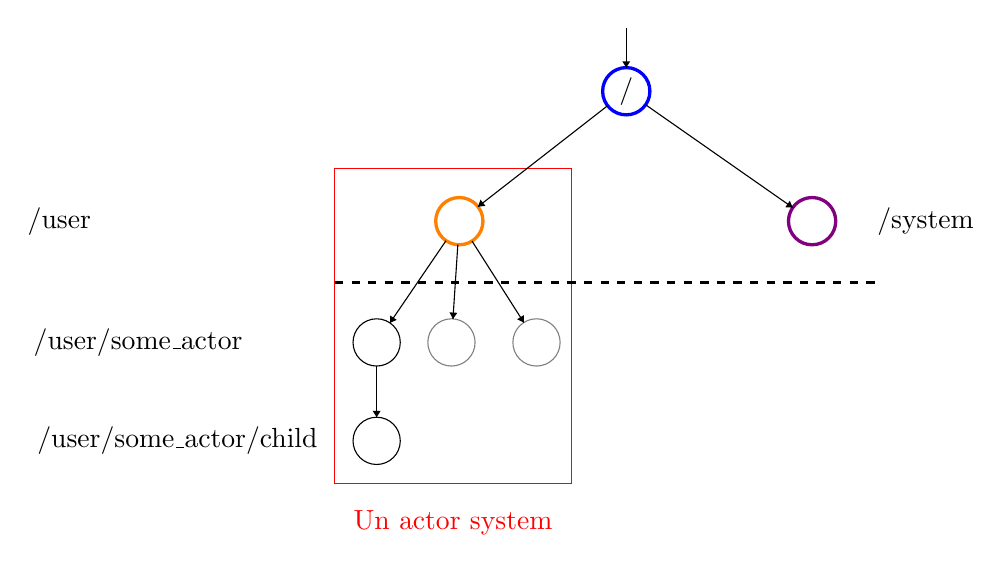
\begin{tikzpicture}[scale=0.1]
	\tikzstyle{every node}+=[inner sep=0pt]
	\draw [blue,very thick] (37,-10.2) circle (3);
	\draw [black] (37,-10.2) node {/};
	\draw [orange,very thick] (15.8,-26.7) circle (3);
	\draw (15.8,-26.7) node {};
	\draw (-35,-26.7) node {/user};
	\draw (75,-26.7) node {/system};
	\draw[red] (0,-20) rectangle (30,-60);
	\draw[red] (15,-65) node {Un actor system};

	\draw (37,-26.7) node {};
	\draw [violet, very thick] (60.6,-26.7) circle (3);
	\draw (60.6,-26.7) node {};
	\draw [black] (5.3,-42.1) circle (3);
	\draw (5.3,-42.1) node {};
	\draw (-25,-42.1) node {/user/some\_actor};
	\draw [gray] (14.8,-42.1) circle (3);
	\draw[thick,dashed] (0,-34.5) -- (69,-34.5);
	\draw (14.8,-42.1) node {};
	\draw [gray] (25.6,-42.1) circle (3);
	\draw (25.6,-42.1) node {};
	\draw [black] (5.3,-54.6) circle (3);
	\draw (5.3,-54.6) node {};
	\draw (-20,-54.6) node {/user/some\_actor/child};
	\draw [white] (26.4,-26.8) circle (3);

	\draw [white] (49.8,-26.7) circle (3);

	\draw [black] (34.63,-12.04) -- (18.17,-24.86);
	\fill [black] (18.17,-24.86) -- (19.11,-24.76) -- (18.49,-23.97);
	\draw [black] (39.46,-11.92) -- (58.14,-24.98);
	\fill [black] (58.14,-24.98) -- (57.77,-24.11) -- (57.2,-24.93);
	\draw [black] (14.11,-29.18) -- (6.99,-39.62);
	\fill [black] (6.99,-39.62) -- (7.85,-39.24) -- (7.03,-38.68);
	\draw [black] (15.61,-29.69) -- (14.99,-39.11);
	\fill [black] (14.99,-39.11) -- (15.55,-38.34) -- (14.55,-38.28);
	\draw [black] (17.41,-29.23) -- (23.99,-39.57);
	\fill [black] (23.99,-39.57) -- (23.98,-38.63) -- (23.14,-39.16);
	\draw [black] (5.3,-45.1) -- (5.3,-51.6);
	\fill [black] (5.3,-51.6) -- (5.8,-50.8) -- (4.8,-50.8);
	\draw [black] (37,-2.2) -- (37,-7.2);
	\fill [black] (37,-7.2) -- (37.5,-6.4) -- (36.5,-6.4);
	\end{tikzpicture}
\end{center}
\caption{Gerarchia del modello ad attori in Akka. In {\color{blue} blu }il \emph{root guardian},
	padre di tutti gli Actor System. In {\color{orange}arancione} il \emph{root user},
	padre di tutti gli user e in fine in {\color{violet}viola} il \emph{system guardian}.}
\end{figure}

\subsection{Scambio di messaggi}
Il protocollo di rete utilizzato per la comunicazione tra i nodi
è \emph{TCP/IP}. Utilizzando tale tipo di protocollo, una volta instaurata
la connessione tra i nodi, il programmatore non si deve preoccupare della
perdita di messaggi o del fatto che possano arrivare non in ordine.

Come protocollo di comunicazione Akka utilizza il \emph{Gossiping};
con l'unica differenza che l'aggiunta di un nuovo membro al cluster viene
inoltrata ai nodi, dando precedenza a quelli che hanno una visione
dello stato meno aggiornata.

Per avere un livello di \emph{location trasparency} discretamente elevato,
abbiamo deciso di non utilizzare la comunicazione diretta tra nodi ma bensì
la indiretta, ovvero un tipo di comunicazione \emph{(time and space)}-\emph{uncoupled}:
 \emph{publish subscribe}.
Come già detto in precedenza, i metodi per la comunicazione indiretta
sono definiti nel package \texttt{akka.cluster.pub-sub.DistributedPubSubMediator}.
La gestione dei gruppi, dei topic e del dispatcher di messaggi è affidata al \emph{mediator};
ogni attore, sia nella fase d'inizializzazione che in qualunque altro momento, potrà informare
il mediator che è interessato ad un determinato topic o che è interessato a ricevere messaggi
da un determinato gruppo di attori. In ogni momento l'attore potrà disiscriversi da un topic o da un gruppo.
 




%%%%%%%%%%%%%%%%%%%%

\subsection{Strutture dati}
Il principale dato che il sistema deve manipolare è un grafo:
la rappresentazione scelta e l'implementazione di tale struttura dati
gioca quindi un ruolo fondamentale. \`E stata data particolare
importanza alla modularità del codice in modo che si possa in seguito
cambiare l'implementazione scelta senza dover modificare l'intero
codice.

L'interfaccia \textbf{\emph{DSGraph}} espone i metodi necessari per
l'algoritmo: la classe \emph{DSGraphImpl} la implementa costituendosi
come wrapper per l'implementazione di basso livello fornita dalla
libreria \emph{graph-stream}. \`E stata scelta tale libreria perché
fornisce diversi metodi per caricare agevolmente il grafo da un file
in formato \texttt{.DOT, .DGS, .GML, .TLP, .NET, .graphML, .GEXF}
e per la sua visualizzazione grafica.
La classe \emph{DSGraphImpl} si occupa anche di gestire internamente
le eccezioni dei metodi della libreria \emph{graphstream} preferendo,
ad esempio,
la restituzione di un valore booleano al lancio di un'eccezione
nel caso di duplice inserimento di uno stesso nodo o arco: questo
rende l'implementazione dei metodi che utilizzano la classe più
flessibile e agevole.
Tuttavia, la libreria non offre metodi per la serializzazione
dei grafi: per poter inviare un grafo in un messaggio è stato
necessario implementare metodi aggiuntivi per serializzare e
de-serializzare il grafo di basso livello in una String.\\
Sono di tipo \emph{DSGraph} il `\emph{mainGraph}' della
\emph{DSDataFacade} e le singole `\emph{myView}' contenute in ogni
robot.

L'interfaccia \textbf{\emph{DSQuery}} estende l'interfaccia
\emph{DSGraph} aggiungendo il metodo \texttt{check-and-reduce()} e la
definizione interna dell'enumerazione \emph{DSQueryStatus},
con i valori \texttt{MATCH, FAIL, DONTKNOW}, e della classe
\textbf{\emph{DSQueryId}}.
Quest'ultima è un wrapper per tre valori la cui
combinazione identifica univocamente una query:~\footnote{
    L'inizializzazione viene fatta dal \emph{DSCluster} quando la
    query viene sottomessa: in particolare il nome viene ricavato
    escludendo il path e l'estensione del file, con l'eventuale
    aggiunta di un numero progressivo nel caso di molteplici
    inserimenti.}
\begin{itemize}
\item un intero `\emph{host}' identificativo del client che ne ha
  richiesto la verifica;
\item una stringa `\emph{name}' ricavata dal nome del file dal quale
  la query è stata caricata;
\item un intero `\emph{nrAttempt}' che numera i tentativi successivi
  per la stessa query nel caso sia terminata in \texttt{DONTKNOW}.
\end{itemize}
Concatenati in una stringa, i tre valori costituiscono il path
identificativo sul quale ascoltano i \emph{DSQueryChecker}
per quella query: opportune manipolazioni della stringa permettono
di estrarre da questo tutti i dati necessari per comunicare
il risultato al \emph{DSClusterInterfaceActor} corretto oppure
per richiedere di presentare nuovamente la query.

La coppia `\emph{host}' e `\emph{name}' è usata come chiave
per l'hash-map `\emph{activeQueries}' (contenuta nel \emph{DSCluster})
che indicizza dei \emph{DSQueryResult}: tale classe è una semplice
coppia di una \emph{DSQuery}, e di una stringa `\emph{stillToVerify}'
corrispondente alla serializzazione della parte ancora da verificare.
Mantenere queste informazioni parziali permette di ritentare la
verifica della query partendo dal risultato intermedio oltre che
far visualizzare all'utente quali parti della query
rimangono sconosciute.\\

Possiamo descrivere le classi dei messaggi scambiati come
wrapper per i dati che contengono:
\begin{itemize}
\item \texttt{DSStartQueryCheck(String serializedQuery,
  DSQueryId id, int TTL)}
\item \texttt{DSCreateQueryChecker(DSQueryId id)}
\item \texttt{DSTryNewQuery(String serializedQuery, int TTL)}
\item \texttt{DSEndQuery(DSQueryId id)}
\item \texttt{DSMissionAccomplished(DSQueryId id,\\
  \phantom{....}
  String serializedStillToVerify, DSQueryStatus status)}
\item \texttt{DSStartCriticalWork(DSQueryId id)}
\item \texttt{DSEndCriticalWork(DSQueryId id)}
\item \texttt{DSRetryQuery(DSQueryId id}
\item \texttt{DSMove()}
\item \texttt{DSRobotFailureOccurred(String deadNode)}
\end{itemize}

La \textbf{\emph{DSDataFacade}}, come già descritto nella
Sezione~\ref{sec:logical-arch}, contiene delle informazioni che devono
essere accessibili da tutto il sistema: è stata dunque implementata
come un singleton accessibile in unica istanza tramite il metodo statico
\texttt{getInstance()}.
Allo stesso modo viene implementato l'accesso alla \emph{DSView} e
ai dati del \emph{DSCluster} da parte del corrispondente
\emph{DSClusterInterfaceActor}.\\

\subsection{Implementazione della view}
\label{sec:viewImpl}
La view (si veda Appendice \ref{sec:view}) è stata realizzata utilizzando \emph{Swing}:
un framework per java appartenente
alla \emph{Java Foundation Class} e orientato allo sviluppo di interfacce grafiche.
La view è composta da tre elementi principali:
\begin{itemize}
	\item Un \emph{JPanel} (\emph{mainPanel}) contenente la rappresentazione
	grafica del grafo etichettato; tale rappresentazione avviene sfruttando le librerie del progetto \emph{graphStream.org (v.1.3)}. Creando un oggetto di tipo \emph{org.graphstream.Graph} e mantenendone il riferimento in memoria, è possibile in qualunque momento modificare le proprietà
	del grafo e ciò ha permesso di poter aggiornare la posizione dei robot ad ogni spostamento.
	\item Un \emph{JTextPane} (\emph{logPane}) contenuto in un \emph{JScrollPane} rappresentante il \emph{log} di sistema; vengono mostrati all'utente: errori nella lettura dei grafi, posizione dei robot e stato della query.
	\item Un \emph{JPanel} (\emph{eastPanelQuery}) anch'esso contenuto in un \emph{JScrollPane} nel quale viene visualizzato lo stato d'avanzamento delle query sottoposte.
\end{itemize}
Inoltre è stato aggiunto un \emph{JMenu} il cui scopo è quello di permettere l'accesso alle impostazioni dell'applicativo.\\

Per migliorare l'attività di debugging è stata aggiunta l'opzione `\emph{auto-move-retry}': nel caso il
risultato di una query fosse \emph{DONTKNOW}, la view inoltra automaticamente al \emph{DSCluster} il comando `\emph{move}' per tutti i robot, seguito dal comando `\emph{retry}'
per la query in questione.
Nel caso in cui l'opzione `\emph{auto-move-retry}' fosse disabilitata, per ogni query presente nell'\emph{eastPanelQuery} verrà visualizzato e abilitato un bottone il cui scopo è quello effettuare
una `\emph{retry}' sulla specifica query.
